% Drawing 29/11-1 -- folder 29, batch 11, archive page 213 (PDF page 214).
% Transcription: en bas à gauche, un petit croquis --- deux ouverts $U$ et $V$ se coupant, avec « $x_1, x_2 \in U$ » --- qui n'est pas repris ici
% Kind: two intersecting open sets U and V. Method 2 (schematic redraw from the facsimile). Status: ok.
% Notes: Two quadrilaterals overlapping: U (thin) and V (heavy), a point in their intersection, labels U, V and "x_1, x_2 in U". The transcription does not reproduce it; redrawn here.
% Coordinates: 1 unit = 1 mm = 1/100 of the crop width (bbox in page fractions: [0.12, 0.74, 0.4, 0.86]).
% Redrawn by Claude (claude-opus-5-5), issue #73, 2026-11-07; not checked by a human; not compiled (no TeX in the session).
% Rights: reproduces part of the work -- behind RENDER_TRANSCRIPTS, never published by itself.
\documentclass[tikz,border=3pt]{standalone}
\usepackage{amsmath,amssymb}
\usetikzlibrary{patterns,arrows.meta}
\tikzset{pencil/.style={black!45}, struck/.style={black!35}, mark/.style={circle,draw,inner sep=1.3pt}, pt/.style={circle,fill,inner sep=0.9pt}, opt/.style={circle,draw,fill=white,inner sep=1.1pt}}
\begin{document}
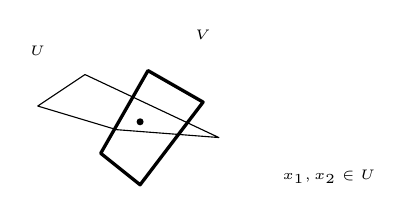
\begin{tikzpicture}[x=1mm,y=1mm,line cap=round,line join=round,font=\scriptsize]
\draw (47,-41) -- (53,-37) -- (70,-45) -- (57,-44) -- cycle;
\draw[very thick] (55,-47) -- (61,-36.5) -- (68,-40.5) -- (60,-51) -- cycle;
\node[pt] at (60,-43) {};
\node[inner sep=1pt] at (47,-34) {\tiny $U$};
\node[inner sep=1pt] at (68,-32) {\tiny $V$};
\node[inner sep=1pt] at (84,-50) {\tiny $x_1, x_2\in U$};
\end{tikzpicture}
\end{document}
